\chapter{Context \& Problem Formulation} \label{chap:problem-formulation}

\begin{chapquote}{\textit{Judea Pearl}}
``As X-rays are to the surgeon, graphs are for causation.''
\end{chapquote}

The main goal of this chapter is to underpin the essential theoretical background and terminology needed to formally define our work:  Causal discovery from time-series data using a foundational neural approach (our LCMs). The purpose of this part is to serve as a conceptual and notational bridge between the high-level motivation discussed in Chapter \ref{chap:introduction} and the following chapters. We focus on Temporal Structural Causal Models (TSCMs) and key assumptions needed for principled causal discovery. Rather than providing a complete treatment of the theory of Causality, our aim is to introduce the necessary formalism tailored to our own setting. For readers seeking a broader perspective on causality, we refer to the seminal works by \citet{pearl2009causality, pearl2018book}, \citet{spirtes2001causation} and \citet{peters2017elements}. For the case of causality and causal discovery in time-series, we point the reader to the works of \citet{runge2018causal, runge2023causal, assaad2022survey, gong2024causal}. We also elaborate on some important aspects of deep learning, as it also serves as an integral part of our work. For a reading on fundamentals, we suggest the textbook by \citet{goodfellow2016deep}. Section \ref{sec:scms} introduces Structural Causal Models, which are then extended to Temporal SCMs (TSCMs) in Section \ref{sec:temp-scms}, while Section \ref{sec:causal-assumptions} outlines the assumptions necessary for causal identifiability and model interpretation. Section \ref{sec:dl} provides a short overview of the necessary deep learning terminology for the unfamiliar reader. Finally, Section \ref{sec:problem-formulation} defines the main objective of our work.


\section{Structural Causal Models} \label{sec:scms}

The framework of Structural Causal Models is fundamental to Causality, as it represents the underlying causal mechanisms that govern an examined system. In order to start formally expressing \textit{\(X \text{ causes } Y\)}, one needs to define the observed variable \(Y\) as a function of \(X \). The notation \(:=\) is introduced to emphasize the asymetric nature of this relationship, rather than merely representing an algebraic equality. That is, \(X\) causes \(Y\), but not vice-versa. In the SCM framework, a variable \(Y\) is modeled as \(Y := f(X, \epsilon)\), where \(f\) is a deterministic (parametric or non-parametric) function, representing the causal mechanism and \(\epsilon\) an exogenous noiseterm which captures, among others, latent, unobserved factors and inherent randomness \citep{peters2017elements}. These noise variables are assumed to be mutually independent across variables and introduce the necessary stochasticity needed to model the causal mechanisms. Assuming no self-causation (a variable causing itself), the relationships between observed variables are qualitatively represented by a \textit{Directed Acyclic Graph (DAG)} where the direct causes of a variable \(X\) are the parents of \(Y\) in the DAG. As such, an edge \(X \rightarrow Y\) in the DAG encodes the causal information that \textit{\(X\) directly causes \(Y\)}. For example, consider the \textit{collider} structure \(X \rightarrow Z \leftarrow Y\), where \(X\) and \(Y\) share the same direct effect. This can be described by the equations \(Z := f(X, Y, \epsilon)\), \( X \sim \epsilon_X, ~Y \sim \epsilon_Y\) where \( \epsilon_X, \epsilon_Y\) are independent noise terms (e.g. sampled from a normal distribution) of \(X\) and \(Y\) respectively. An illustration is shown in Figure \ref{fig:scm}. If one ignores any causal interpretation of the functional mechanisms, this representation turns into a \textit{Structural Equation Model (SEM)}. Formally, we define an SCM as a tuple of (i) a set of \textit{endogenous} variables \(\mathcal{V}\), a set of \textit{exogenous} variables \(\mathcal{U}\) and the set \(\mathcal{F}\) of functions of the form \( f \equiv f(\text{Pa}(V_i),\epsilon_i)\), where \(\text{Pa}(V_i)\) denotes the direct causes of \(V_i\) (parents of \(V_i\) in the DAG), to generate each endogenous variable as a function of other variables. In practice, the functions \(f_i\) are often assumed to follow the form of an \textit{additive noise model (ANM)}. In this, case, the functional relationships are of the form 

\begin{equation}
    V_i := f(\text{Pa}(V_i), \epsilon_i) = f(\text{Pa}(V_i)) + \epsilon_i
\end{equation}

which simplifies estimation and data generation, while still allowing for representing a rich class of linear and non-linear causal mechanisms. In a nutshell, this serves as just another assumption to facilitate causal identifiability and inference.

\begin{figure}[t!]
\centering
\begin{minipage}{0.55\textwidth}
\centering
\begin{tikzpicture}[>=Stealth, node distance=1.2cm, every node/.style={circle, draw, minimum size=6mm, thick, font=\small}]		

% Nodes
\node (E1) [dashed] {$\epsilon_1$};
\node (X1) [below=of E1,yshift=0.4cm] {$X_1$};
\node (E2) [right=1.5cm of X1, dashed] {$\epsilon_2$};
\node (X2) [below=of E2,yshift=0.4cm] {$X_2$};
\node (E3) [left=1.5cm of X1, dashed] {$\epsilon_3$};
\node (X3) [below=of E3,yshift=0.4cm] {$X_3$};

% Edges
\draw[->, thick] (E1) -- (X1);
\draw[->, thick] (E2) -- (X2);
\draw[->, thick] (E3) -- (X3);
\draw[->, thick] (X1) -- (X2);
\draw[->, thick] (X1) -- (X3);

\end{tikzpicture}
\end{minipage}%
\hfill
\begin{minipage}{0.4\textwidth}
\centering
\vspace{1em}
\[
\begin{array}{l}
X_1 = f_1(\epsilon_1) \\[0.5em]
X_2 = f_2(X_1,\, \epsilon_2) \\[0.5em]
X_3 = f_3(X_1,\, \epsilon_3)
\end{array}
\]
\end{minipage}
\caption{Illustration of Structural Equation Model for an inverse collider structure \( X \leftarrow Z \rightarrow Y\). Each variable is a function of its direct causes and a noise term.} \label{fig:scm}
\end{figure}


\section{The Temporal Setup} \label{sec:temp-scms}

The case for time-series data can be seen an a natural generalization of the above, but taking into account the additional temporal dimension of data. Let \( \left\{ \mathbf{V}_t \right\}_{t \in \mathbb{Z}} \) denote a multivariate stochastic process, with \(V_t=(V^1_t,\ldots,V^N_t)\) representing the state of the system at time \(t\). A \textit{Temporal Structural Causal Model (TSCM)} consists of the structural assignments

\begin{equation} \label{eq:scm}
V^j_t \;:=\; f_j\bigl(\text{Pa}(V^j_t),\,\epsilon^j_t\bigr), ~\quad j=1,\dots,N,\;\;t\in\mathbb{Z},
\end{equation}

where for each variable index \(j\), \(\epsilon^j_t\) is an independent exogenous noise term, \( \text{Pa}(V^j_t)\;\subseteq\;\{V^i_{t-\tau}:i=1,2,\ldots,N,\;\tau=0,\ldots,,\ell_{\max}\}\setminus\{V^j_t\} \) denotes the \emph{causal parents} of \(V^j_t\) occurring at the same (if the existence of contemporaneous effects is assumed) or earlier time steps \(t-1,t-2,\ldots\), up to a finite maximal lag \(\ell_{\max}> 0\). Analogously to the atemporal case, each function \( f^j\) is the functional deterministic causal mechanism that determines the value of \(V^j_t\) given the direct causes \( \text{Pa}(V^j_t)\) and the corresponding noise term \(\epsilon^j_t\). The TSCM can then be written as a tuple \((\mathcal{G},\mathcal{F}, \mathcal{E})\) where \(\mathcal{G}\) is the causal graph, \(\mathcal{F}\) is the set of functional dependencies \(f^j\) and \(\mathcal{E}\) is the set of noise terms \(\epsilon^j_t\).  

The causal parents \(\text{Pa}(V^j_t)\), also called \textit{direct causes}, are selected from the set \(\{V^j_t, \ldots,  V^j_{t-\ell_\text{max}}\}\). This formalism encodes both lagged and contemporaneous causal effects (\(\ell_\text{max} = 0\)) to be represented, making it suitable for modeling a wide range of dynamical systems. To ensure well-posedness, we restrict all parent sets to occur at most \( \ell_\text{max} \) time-steps in the past, thus disallowing backward in-time causation. Recall that contemporaneous edges \(V^i_t \rightarrow V^j_t\) may occur if causal effects exist beyond the presumptive granularity (e.g. hourly causal mechanisms against a daily assumed lag). Furthermore, it is assumed that the temporal process is governed by a finite horizon of causal interactions and that each variable has a bounded number of causal inputs. Again, the functional relationships between the observed variables are represented by a DAG where edges move forward in time. As a concrete example, consider an observed process with the time-series \( V^1, V^2\) and \(V^3\) with the following causal relationships: Variable \(V^1\) directly causes variable \(V^2\) with lag \(1\) and \(V^2\) directly causes \(V^3\) with lag \(2\). As the process extends through time, so do the edges of the causal graph. The process (and as such the causal edges) may evolve, which makes the causal graph time-dependent. That is, different causal graphs may correspond to different time horizons and time windows. This pivots towards our first definition of the most important causal assumption for time-series data: \textit{Causal Stationarity}.

\begin{definition}[Causal Stationarity, \cite{runge2018causal}] Consider an SCM described as in Equation \ref{eq:scm}. If the causal relationships between variables \((V^i_{t-\tau}, V^j_t )\) for lag \(\tau>0\) also hold for all time-shifted versions \((V^i_{t' -\tau}, V^j_{t'}) \), the described process is \textit{causally stationary}. Informally, the graph structure and noise distribution of the SCM are time-invariant.
\end{definition}

Using the previous example, that means that, for the current timepoint \(t\), there exist causal edges such as \( V^1_{t-1} \rightarrow V^2_t \) and \( V^2_{t-2} \rightarrow V^3_t \). By causal stationarity, these relations also hold for their time-shifted versions: \( V^1_{t'-1} \rightarrow V^2_{t'} \) and \( V^2_{t'-2} \rightarrow V^3_{t'} \) for all \( t' \leq t \). Like in the atemporal case, indirect causation is implied through directed paths. In literature, this invariance of causal effects in time is also referred to as time homogeneity \citep{gong2024causal}.

The causal dependencies implied by a TSCM can be visualized as a directed graph unrolled over time. The cautious reader may have observed that due to the temporal axis, multiple graph abstractions are possible depending on the intended level of granularity. We first define the most complete representation, the \textit{full-time causal graph}:

% Full Time Causal Graph (a)
\begin{figure}[t!]
\centering
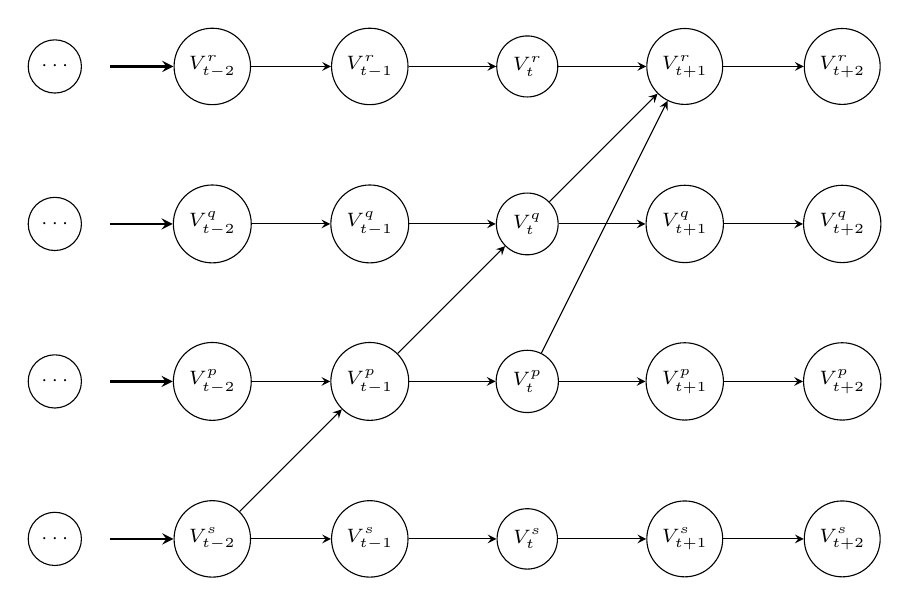
\begin{tikzpicture}[
    every node/.style={circle, draw, minimum size=0.5cm, font=\scriptsize},
    >=stealth,
    ->,
]

% Coordinates and ellipsis
\foreach \i/\y in {r/6, q/4, p/2, s/0} {
    % Main nodes from t-2 to t+2
    \foreach \j/\x in {-2/-4, -1/-2, 0/0, 1/2, 2/4} {
        \node (\i\j) at (\x,\y) {$V^{\i}_{t\ifnum\j<0 \j\else\ifnum\j=0 \else+\j\fi\fi}$};
    }
    % Dots on the far left
    \node at (-6,\y) {$\cdots$};
    % Arrows from dots to first node
    \draw[->, thick] (-5.3,\y) -- (\i-2);
}

% Temporal self-links
\foreach \i in {r,q,p,s} {
    \foreach \j/\k in {-2/-1, -1/0, 0/1, 1/2} {
        \draw (\i\j) -- (\i\k);
    }
}

% Cross-temporal causal edges
\draw (s-2) -- (p-1);
\draw (p-1) -- (q0);
\draw (q0) -- (r1);
\draw (p0) -- (r1);

\end{tikzpicture}
\caption{Full time causal graph: The temporal SCM extends infinitely into the past (indicated by \(\cdots\) and incoming arrows) and shows both auto- and cross-variable lagged dependencies. Notice that in this example, no causal stationarity is assumed.}
\label{fig:full-time-causal-graph}
\end{figure}

\begin{definition}[Full-Time Causal Graph]
Let \(\left\{ \mathbf{V}_t \right\}_{t \in \mathbb{Z}}\) be a multivariate stochastic process governed by a Temporal SCM. The \textit{full-time causal graph} is the infinite directed acyclic graph (DAG) whose nodes are all variables \(V^i_t\) for every \(i \in \{1, \dots, N\}\) and every time step \(t \in \mathbb{Z}\), and whose edges correspond to direct causal relationships \(V^i_{t - \tau} \rightarrow V^j_t\) as defined by the TSCM. This graph includes both within-variable (autoregressive) and cross-variable temporal dependencies across all lags up to \(\ell_{\max}\).
\end{definition}

Figure \ref{fig:full-time-causal-graph} illustrates such a structure, where both temporal self-dependencies and cross-variable influences are made explicit. This infinite graph represents the most faithful unfolding of the SCM in time. If causal stationarity is not assumed (as illustrated), then different causal graphs correspond to different time horizons, further complicating the causal discovery task. Secondly, the full-time causal graph can be truncated to a specific time-horizon, resulting in the \textit{time-lagged (also called \textit{windowed}) causal graph}, with causal edges up to \(\ell_\text{max}\). 

\begin{definition}[Lagged Causal Graph - Window Causal Graph]
A \textit{lagged causal graph} is a directed acyclic graph (DAG) that represents causal relationships between time-shifted variables in a multivariate time-series. Formally, let \(\mathbf{V}_t = \{V^1_t, V^2_t, \dots, V^k_t\}\) denote the set of observed variables at time step \(t\). A lagged causal graph \(\mathcal{G}\) contains directed edges of the form \(V^i_{t-\tau} \rightarrow V^j_t\), where \(\tau \in \{1, 2, \dots, \ell_{\max}\}\) is a positive time lag. An edge \(V^i_{t-\tau} \rightarrow V^j_t\) indicates that \(V^i\) is a direct cause of \(V^j\) with a time lag of \(\tau\).
\end{definition}

An example of a lagged causal graph is illustrated in Figure \ref{fig:temporal-graphs} (a). Finally, the lagged causal graph can be further simplified to a more concise representation, the \textit{summary causal graph}.

\begin{definition}[Summary Causal Graph]
 Given a lagged causal graph \(\mathcal{G}\) with edges of the form \(V^i_{t-\tau} \rightarrow V^j_t\) for various lags \(\tau\), the corresponding summary graph \(\mathcal{S}\) contains an edge \(V^i \rightarrow V^j\) if there exists at least one lag \(\tau\) such that \(V^i_{t-\tau}\) is a direct cause of \(V^j_t\) in \(\mathcal{G}\).
\end{definition}

Essentially, a summary graph is a simplified representation of the lagged causal structure in a time-series, where the temporal information about lags is abstracted away, as shown in Figure \ref{fig:temporal-graphs} (b). The summary graph collapses temporal information and only displays whether a causal relationship exists between two variables, but it does not specify the lag or delay at which the causal influence occurs. Note that from a lagged causal graph one can obtain the summary graph (e.g. from Figure \ref{fig:temporal-graphs} (a) to Figure \ref{fig:temporal-graphs} (b)), but not vice-versa, as the lag of causal relationships is not encoded in the summary structure. Summary graphs that retain temporal information can of course be obtained from the lagged causal graph, but remain outside the scope of our text.   

\begin{figure}[t!]
\centering

% Lagged and Summary Graph Side-by-Side
\begin{minipage}[t]{0.48\textwidth}
\centering
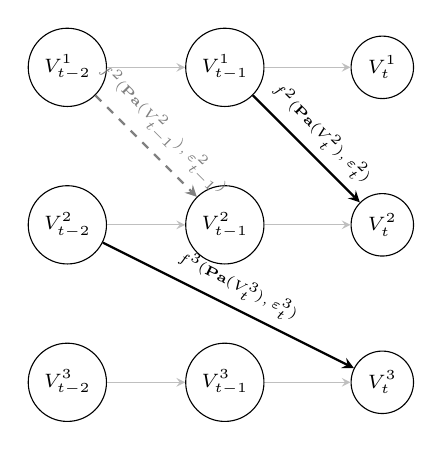
\begin{tikzpicture}[
    varnode/.style={circle, draw, minimum size=0.6cm, font=\scriptsize},
    >=stealth,
    ->,
    dashededge/.style={->, dashed, thick, color=gray},
    solidedge/.style={->, thick},
]

% t-2
\node[varnode] (V1t2) at (0,4) {$V^1_{t-2}$};
\node[varnode] (V2t2) at (0,2) {$V^2_{t-2}$};
\node[varnode] (V3t2) at (0,0) {$V^3_{t-2}$};

% t-1
\node[varnode] (V1t1) at (2,4) {$V^1_{t-1}$};
\node[varnode] (V2t1) at (2,2) {$V^2_{t-1}$};
\node[varnode] (V3t1) at (2,0) {$V^3_{t-1}$};

% t
\node[varnode] (V1t) at (4,4) {$V^1_{t}$};
\node[varnode] (V2t) at (4,2) {$V^2_{t}$};
\node[varnode] (V3t) at (4,0) {$V^3_{t}$};

% Optional: temporal arrows (light gray)
\foreach \i in {1,2,3} {
  \draw[->, gray!50] (V\i t2) -- (V\i t1);
  \draw[->, gray!50] (V\i t1) -- (V\i t);
}

% Causal arrows with functional labels directly on edges
\draw[solidedge] (V1t1) -- (V2t)
  node[midway, above, sloped, font=\tiny, draw=none, fill=none] 
  {$f^{2}(\mathbf{Pa}(V^2_t),\varepsilon^2_t)$};

\draw[dashededge] (V1t2) -- (V2t1)
  node[midway, above, sloped, font=\tiny, draw=none, fill=none] 
  {$f^{2}(\mathbf{Pa}(V^2_{t-1}),\varepsilon^2_{t-1})$};

\draw[solidedge] (V2t2) -- (V3t)
  node[midway, above, sloped, font=\tiny, draw=none, fill=none] 
  {$f^{3}(\mathbf{Pa}(V^3_t),\varepsilon^3_t)$};

\end{tikzpicture}


\vspace{0.5em}
{(a) Lagged causal graph}
\end{minipage}
\hfill
\begin{minipage}[t]{0.48\textwidth}
\centering
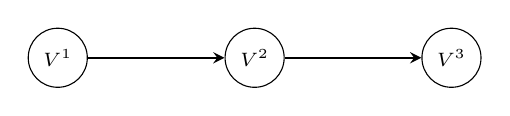
\begin{tikzpicture}[
    every node/.style={circle, draw, minimum size=0.6cm, font=\scriptsize},
    >=stealth,
    ->,
]

\node (V1) at (2,2) {$V^1$};
\node (V2) at (4.5,2) {$V^2$};
\node (V3) at (7,2) {$V^3$};

\draw[->, thick] (V1) -- (V2);
\draw[->, thick] (V2) -- (V3);

\end{tikzpicture}

\vspace{0.5em}
{(b) Summary causal graph}
\end{minipage}

\caption{Illustration of a temporal SCM with max lag \(\ell_{\max}=2\). (a) The lagged causal graph shows variable \(V^1\) causing \(V^2\) with lag 1 and \(V^2\) causing \(V^3\) with lag 2. Dashed edges encode the assumption of causal stationarity, meaning that the same causal dependencies recur over time. Functional dependencies between lagged variables are shown directly on the edges. (b) The summary causal graph discards time lag information, representing only the aggregated causal influences.}
\label{fig:temporal-graphs}
\end{figure}

\section{Probabilistic Quantifications} \label{sec:bns}

To introduce our next causal assumptions, one needs to understand how causal structures relate to probabilistic reasoning, by the formalism of \textit{Bayesian networks (BNs)}. BNs provide a compact representation of a joint probability distribution using a directed acyclic graph. Each node corresponds to a random variable, and each directed edge represents a statistical dependence.

Briefly, a Bayesian network is defined as a pair \((\mathcal{G}, \mathbb{P})\), where \(\mathcal{G} = (\mathbf{V}, \mathcal{E})\) is a DAG with nodes \(\mathbf{V} = \{X_1, \dots, X_n\}\), and \(\mathbb{P}\) is a joint distribution over \(\mathbf{V}\), which factorizes, according to the chain rule, based on the structure of \(\mathcal{G}\). That is, each variable \(X_i\) is conditionally independent of its non-descendants given its parents \(\mathrm{Pa}(X_i)\) in the graph:

\begin{equation}
\mathbb{P}(X_1, \dots, X_n) = \prod_{i=1}^n \mathbb{P}(X_i \mid \mathrm{Pa}(X_i)).
\end{equation}

This factorization, which \citet{bengio2019meta} call \textit{disentangled factorization}, provides both computational efficiency and semantic clarity: each conditional distribution models a local dependency, and the global distribution emerges from their composition. Compared to SCMs which explicitly model causal mechanisms through assignments \(X_i := f_i(\mathrm{Pa}(X_i), \epsilon_i)\), BNs represent probabilistic dependencies only. While every SCM induces a Bayesian Network (through the distribution entailed by its noise and mechanisms), the converse does not hold; Bayesian Networks may not capture the directionality or manipulability implied by causality, so interventions and counterfactuals are not applicable. If one assumes causal interpretation on the edges, the resulting BN can be treated as a \emph{causal BN}. In a nutshell, the key advantage of Bayesian Networks lies in their ability to encode and reason about conditional independencies, which are central to many causal discovery approaches.


\section{Causal Assumptions} \label{sec:causal-assumptions}

We now elaborate on causal assumptions needed for performing identifiability of the true causal graph and consequently, sound causal inference. We have already elaborated on the assumption of causal stationarity in Section \ref{sec:temp-scms}. All causal discovery algorithms are governed by a set of assumptions, regarding the statistical properties of the data and the underlined structure of the causal model. Is is thus evident that making and understanding causal assumptions is also vital for correct interpretation not only of the discovered causal structure. We define the following assumptions in a way to be applied to either a (standard) causal graph or analogously to a temporal causal graph.

\begin{definition}[Causal Markov Condition, \citep{spirtes2001causation}] Let \(\mathcal{G}\) be a causal graph with vertex set \(\mathbf{V}\) and \(\mathbb{P}\) a probability distribution over \(\mathbf{V}\), generated by the causal structure induced by \(\mathcal{G}\). Then \(\mathcal{G}\) and \(\mathbb{P}\) satisfy the Markov Condition if and only if \(~\forall ~W \in \mathbf{V}\), \(W\) is independent of its non-descendants (non causal effects) given its parents (direct causes) on \(\mathcal{G}\).
\end{definition}

Essentially, the Causal Markov Condition assures that conditional independences between variables are exactly those entailed by the causal graph (i.e. by d-separation).

\begin{definition}[Faithfulness, \citep{spirtes2001causation}] Let \(\mathcal{G}\) be a causal graph and \(\mathbb{P}\) a probability distribution over \(\mathbf{V}\). We say that \(\mathcal{G}\) and \(\mathbb{P}\) are faithful to each other if and only if (iff) the all and only the independence relations of \(\mathbb{P}\) are entailed by the Causal Markov condition of \(\mathcal{G}\). Specifically, \(\mathcal{G}\) and \(\mathbb{P}\) satisfy the Faithfulness Condition if-f every conditional independence relation true in \(\mathbb{P}\) is entailed by the Causal Markov Condition applied to \(\mathcal{G}\).
\end{definition}

In other words, given a causally sufficient set of variables \(\mathcal{U}\) in a population \(N\), \textit{every} conditional independence relation that holds in the density over \(\mathcal{U}\) \textit{is entailed by the local directed Markov condition for the causal DAG of \(N\)}. The key argument behind assuming faithfulness of the true causal graph and the corresponding distribution induced by observed data is that non-faithfulness would lead to determinism in the observed system. As everything would cause everything and no stochasticity is involved, performing causal queries would prove invalid.  

\begin{definition}[Causal Sufficiency, \citep{spirtes2001causation}] A set \(\mathbf{V}\) of variables is causally sufficient for a population iff in the population every common cause of any two or more variables in \(\mathbf{V}\) is in \(V\), or has the same value for all units in the population. The common cause \(Z\) of two or more variables in a DAG \(X \leftarrow Z \rightarrow Y\) is called a \textit{confounder of \(X\) and \(Y\)}. Hence causal sufficiency implies no unobserved confounders. The notion of causal sufficiency is being used without explicitly mentioning the population.
\end{definition}

\begin{figure}[ht!]
\begin{multicols}{2}
	\begin{center}
		\begin{tikzpicture}[->,>=stealth,thick]
			% X -> L -> Y
			\node[draw, circle] (XLY1) {$X$};
			\node[draw, rectangle,right=of XLY1] (L1) {$L$};
			\node[draw, circle,right=of L1] (Y1) {$Y$};
			
			\draw[->] (XLY1) -- (L1);
			\draw[->] (L1) -- (Y1);
		\end{tikzpicture}
	\columnbreak

		\begin{tikzpicture}[->,>=stealth,thick]
			% X <-> Y
			\node[draw, circle] (XY1) {$X$};
			\node[draw, circle,right=of XY1] (Y1) {$Y$};
			
			\draw[->] (XY1) -- (Y1);
		\end{tikzpicture}
	\end{center}
\end{multicols}

\begin{multicols}{2}
	\begin{center}
		\begin{tikzpicture}[->,>=stealth,thick]
			% X <-> L <-> Y
			\node[draw, circle] (XLY2) {$X$};
			\node[draw, rectangle,right=of XLY2] (L2) {$L$};
			\node[draw, circle,right=of L2] (Y2) {$Y$};
			
			\draw[<-] (XLY2) -- (L2);
			\draw[<-] (L2) -- (Y2);
		\end{tikzpicture}
	
	    \columnbreak
	    
		\begin{tikzpicture}[->,>=stealth,thick]
			% X <-> Y
			\node[draw, circle] (XY2) {$X$};
			\node[draw, circle,right=of XY2] (Y3) {$Y$};
			
			\draw[<-] (XY2) -- (Y3);
		\end{tikzpicture}
	\end{center}
\end{multicols}

\begin{multicols}{2}
		\begin{center}
		\begin{tikzpicture}[->,>=stealth,thick]
			% X <-> L <-> Y
			\node[draw, circle] (XLY2) {$X$};
			\node[draw, rectangle,right=of XLY2] (L2) {$L$};
			\node[draw, circle,right=of L2] (Y2) {$Y$};
			
			\draw[->] (XLY2) -- (L2);
			\draw[<-] (L2) -- (Y2);
		\end{tikzpicture}
	\end{center}
    \columnbreak
	\begin{center}
		\begin{tikzpicture}[->,>=stealth,thick]
			% X <-> Y
			\node[draw, circle] (XY2) {$X$};
			\node[draw, circle,right=of XY2] (Y3) {$Y$};
			
		\end{tikzpicture}
	\end{center}
\end{multicols}

\begin{multicols}{2}
	\begin{center}
		\begin{tikzpicture}[->,>=stealth,thick]
			% X <-> L <-> Y
			\node[draw, circle] (XLY2) {$X$};
			\node[draw, rectangle,right=of XLY2] (L2) {$L$};
			\node[draw, circle,right=of L2] (Y2) {$Y$};
			
			\draw[<-] (XLY2) -- (L2);
			\draw[->] (L2) -- (Y2);
		\end{tikzpicture}
	\end{center}
	
	\columnbreak
	
	\begin{center}
		\begin{tikzpicture}[->,>=stealth,thick]
			\node[draw, circle] (XY2) {$X$};
			\node[draw, circle,right=of XY2] (Y3) {$Y$};
			\node at (0.9,0) {?};
		\end{tikzpicture}
	\end{center}
\end{multicols}
\caption{Illustrations for the presence of a hidden confounder \(L\) for two variables \(X,Y\), in the case of atemporal data. In the first case, where \(X\) indirectly causes \(Y\) with \(L\) acting as a mediator, we observe that \(Dep(X,Y)\) so we infer \(X \rightarrow Y\), and similarly \(X \leftarrow Y\) in the second case. In the third case where \(X\) and \(Y\) share a hidden common effect, we infer \(Indep(X,Y)\) and thus discover no edge between \(X\) and \(Y\). However, in the case of \(L\) being a hidden common cause of \(X\) and \(Y\), there exists no DAG that captures the dependencies.}
\label{fig:dag-conf}
\end{figure}

To put it simply, causal sufficiency is the \textit{asumption of no unobserved variables}. Unobserved variables are called \textit{latent} or \textit{hidden}. The fact that DAGs are unable to adequately capture latent confounders becomes apparent in the example at Figure \ref{fig:dag-conf}, for the case of i.i.d. data. The assumption can be adapted similarly for the case of time-series, where one can assume latent confounders may exist at a predefined time-lag. For example \(V^1_{t}\) and \(V^2_{t}\) may be confounded by the latent variable \(V^3_{t-1}\). SCMs without unobserved confounders are also called \textit{Markovian models} as the noise terms of the variables are independent. The observed variables in SCMs with unobserved confounding can have dependent noise terms, called \textit{semi-Markovian models}.

It must be noted that in practice, not all variables in the underlying SCM are measured. A projected causal graph on the observed subset is represented as an \textit{Acyclic Directed Mixed Graph} (ADMG), in which a bidirected arrow \(V^i_{t-\tau}\leftrightarrow V^j_t\) indicates the presence of an unobserved common cause with lag \(\tau\). For atemporal data, causal structures that enable marginalization of an SCM (a model with a subset of variables) exist \citep{richardson2002ancestral}, but remain completely outside our scope. This formulation also underlies algorithms for causal discovery under latent confounding, or when inferring contemporaneous effects where directionality is unknown.

\begin{figure}[h]
\centering
\begin{tikzpicture}[
    every node/.style={circle, draw, minimum size=0.6cm, font=\scriptsize},
    >=stealth,
    ->,
    solidedge/.style={->, thick},
    removededge/.style={->, red, dotted, thick, opacity=0.5},
    interbox/.style={rectangle, draw, minimum width=0.5cm, minimum height=0.4cm, font=\tiny, fill=black!5}
]

% Nodes at t-2
\node (V1t2) at (0,6) {$V^1_{t-2}$};
\node (V2t2) at (0,4) {$V^2_{t-2}$};
\node (V3t2) at (0,2) {$V^3_{t-2}$};

% Nodes at t-1
\node (V1t1) at (3,6) {$V^1_{t-1}$};
\node (V2t1) at (3,4) {$V^2_{t-1}$};
\node (V3t1) at (3,2) {$V^3_{t-1}$};

% Nodes at t
\node (V1t) at (6,6) {$V^1_{t}$};
\node (V2t) at (6,4) {$V^2_{t}$};
\node (V3t) at (6,2) {$V^3_{t}$};

% Temporal identity edges (gray)
\foreach \i in {1,2,3} {
  \draw[->, gray!50] (V\i t2) -- (V\i t1);
  \draw[->, gray!50] (V\i t1) -- (V\i t);
}

% Causal edges
\draw[->, gray!50] (V1t2) -- (V3t1);     % V^1_{t-2} -> V^3_{t-1}
\draw[solidedge] (V1t1) -- (V3t);        % V^1_{t-1} -> V^3_t
\draw[->, gray!50] (V2t2) -- (V3t1);     % V^2_{t-2} -> V^3_{t-1}
\draw[solidedge] (V2t1) -- (V1t);        % V^2_{t-1} -> V^1_t
\draw[solidedge] (V2t1) -- (V3t);        % V^2_{t-1} -> V^3_t

% Removed incoming edges to V1_{t-1}
\draw[removededge] (V1t2) -- (V1t1);     % V^1_{t-2} -> V^1_{t-1} (self-dependence, optional)
\draw[removededge] (V2t2) -- (V1t1);     % V^2_{t-2} -> V^1_{t-1}

% Intervention label
\node[interbox, right=2pt of V1t1] {\scriptsize do($V^1_{t-1}$)};

\end{tikzpicture}
\caption{A dense lagged causal graph with an intervention on \( V^1_{t-1} \), where \(V^2\) directly causes \(V^1\) \& \(V^3\) with lag 1 and \(V^1\) directly causes \(V^3\) with lag 1. The intervention \( \text{do}(V^1_{t-1}) \) removes all incoming edges to \( V^1_{t-1} \), shown as red dotted lines, while preserving its downstream influence on \( V^3_t \). The interventional value replaces the natural dynamics of \( V^1_{t-1} \), breaking any backdoor paths through its original causes.
}
\label{fig:interv-example}
\end{figure}

As we have seen in Chapter \ref{chap:introduction}, the first rung that differentiates a probabilistic model with a causal model is the ability to perform interventions, that is, modifying the internal causal mechanisms of the examined system. We define interventions for the temporal setting, which only differs in the temporal dimension of the variables. TSCMs allow interventions to be performed in a simple manner: Modify the structural assignment in the SCM of a variable \(X^k\) to \(x\). This corresponds to a \textit{hard intervention} at a specific timestep \(t\). The resulting interventional distribution \(\mathbb{P}(Y_t|\text{do}(X^k_t=x))\) captures the causal effect of setting \(X\) to \(x\). The reader should recall that the observational and interventional distributions may differ because non-causal associations (e.g., due to confounders) are blocked under interventions. In the causal graph, this corresponds to performing \textit{graph surgery}, by removing all incoming edges to \(X^k_t\) and replacinb the structural equation with \(X^k_t:=x\), due to what is known as the \textit{modularity assumption}. An example is illustrated in Figure \ref{fig:interv-example}. One may also apply different interventions to different variables \(X^i_t, X^j_t\), (\textit{multiple interventional targets}) at the same timestep, resulting in an interventional distribution \( \mathbb{P}(Y_t | \text{do}(X^i_t=x^i_t, X^j_t=x^j_t))\). For soft interventions, as the name may suggest, instead of explicitely modifying the structural assignment, one adds a noise term (either sampled from a known parametric distribution like a Gaussian, or sampled from a prior distribution) to the structural assignment. Consequently, interventions allow us to define causality in a much more rigid manner: A variable \(X^i\) causes \(X^j\) if an intervention on \(X^i\) leads to a direct change in \(X^j\). Conclusively, do-calculus provides a set of transformation rules to express interventional (and counterfactual, although outside of our scope) distributions in terms of observable quantities, given a true or discovered causal graph. It underpins identification results, determining whether a causal effect can in principle be recovered from observational data alone or whether additional assumptions or interventional data are required. For causal discovery algorithms, handling of interventional data leads further into correct identifiability of the true causal graph, which may not be possible with observational data alone. 

\section{Brief Deep Learning Overview} \label{sec:dl}

This section aims to provide a high-level overview of deep learning for the unfamiliar reader, which is the second important pillar our work is based on. 

The backbone of deep learning is the concept of \textit{artificial neural network (ANN)}, abbreviated as neural network (NN). Such a network consists of a collection of connected units named neurons. The name stems from the introduction of the first model, Rosenblatt's Multilayer Perceptron (MLP) \citep{rosenblatt1958perceptron}, which loosely mimics the connection of biological neurons in the brain. Each neuron is connected to other neurons like a synapse in the brain, with signal being propagated throught the network using weights associated with the connections, which are real numbers. The larger the number, the stronger the connection.

\begin{figure}[h]
    \centering
    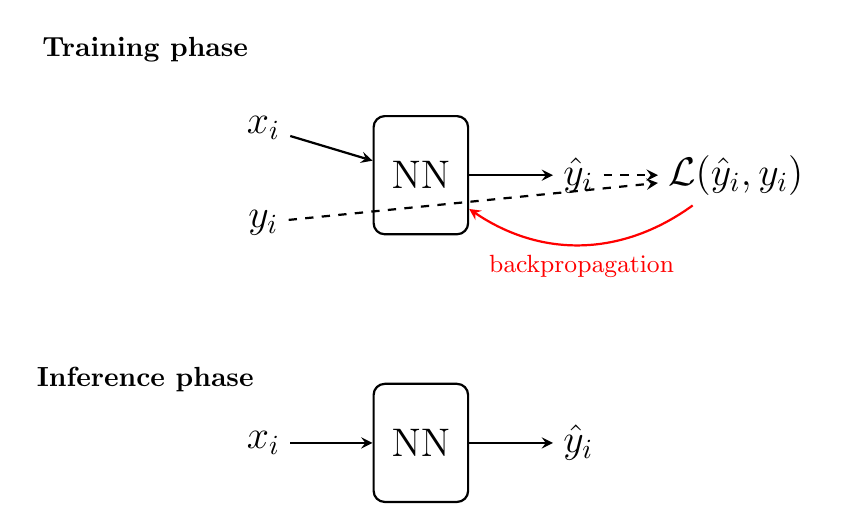
\begin{tikzpicture}[>=stealth, thick, node distance=1.8cm]
        % Training phase
        \node at (-1.5, 2) {\textbf{Training phase}};
        \node (xtrain) at (0,1) {\Large $x_i$};
        \node (ytrain) at (0,-0.2) {\Large $y_i$};
        \node[draw, rounded corners, minimum width=1.2cm, minimum height=1.5cm] (nntrain) at (2,0.4) {\Large NN};
        \node (yhattrain) at (4,0.4) {\Large $\hat{y}_i$};
        \node (loss) at (6,0.4) {\Large $\mathcal{L}(\hat{y}_i, y_i)$};

        % Training arrows
        \draw[->] (xtrain) -- (nntrain);
        \draw[->] (nntrain) -- (yhattrain);
        \draw[->, dashed] (ytrain) -- (loss);
        \draw[->, dashed] (yhattrain) -- (loss);
        \draw[->, thick, red] (loss) to[bend left=35] node[midway, below] {\small backpropagation} (nntrain);
        % Inference phase
        \node at (-1.5, -2.2) {\textbf{Inference phase}};
        \node (xtest) at (0,-3) {\Large $x_i$};
        \node[draw, rounded corners, minimum width=1.2cm, minimum height=1.5cm] (nntest) at (2,-3) {\Large NN};
        \node (yhattest) at (4,-3) {\Large $\hat{y}_i$};
        % Inference arrow
        \draw[->] (xtest) -- (nntest);
        \draw[->] (nntest) -- (yhattest);

    \end{tikzpicture}
    \caption{Illustration of neural network training and inference. During training, both input-output pairs \((x_i, y_i)\) are provided to compute the loss \(\mathcal{L}(\hat{y}_i, y_i)\) and update model parameters via backpropagation. During inference, only the input \(x_i\) is given, and the trained network produces an estimated output \(\hat{y}_i\).}
    \label{fig:nn-train-infer}
\end{figure}

Similarly to supervised learning algorithms, a neural network assumes a data input and constructs an output, based on a collection of data instances, in order to find a suitable representation between them, via a process called \textit{training}. By processing such ground truth input and output pairs, training the model employs a \textit{supervised learning scheme} (see Figure \ref{fig:nn-train-infer}). In practice, training the model refers to adjusting its set of trainable parameters (such as the weight between neurons as illustrated before) in order to find the relationship between the input and target data pairs (assuming it exists). Training such a model consists of numerous important steps. As training consists of a mathematical optimization approach (since the problem is intractable), the goal is to minimize an objective function (loss function) that measures the error in performance, often as the absolute difference between the model's estimated outputs and the ground truth targets. Minimization of such a function is attained by the adjustment of the trainable parameters, which occurs iteratively as dictated by the training \textit{optimizer}, based on gradients computed through \textit{backpropagation} \citep{lecun1988theoretical, werbos2002backpropagation}. Backpropagation applies the chain rule of calculus in reverse (illustrated in Figure \ref{fig:building-blocks}), computing how much each parameter contributed to the error signal. This allows the optimizer to make informed adjustments. Common optimizers include Stochastic Gradient Descent (SGD) \citep{ruder2016overview} and Adam \citep{kingma2015adam}, both of which aim to efficiently navigate the high-dimensional loss landscape.

Once trained, the model can generalize to unseen data in the \textit{inference phase}, where it takes only input \(x_i\) and outputs a prediction \(\hat{y}_i\). Neural network models are known as universal approximators \citep{hornik1989multilayer}. This illustrates that in cases where statistical, machine learning, or even very simple methods fail due to the intractable nature of the function \(f\) between input and output, it becomes significant to consider fitting a neural network model.

Progress in neural networks and deep learning has often been driven by the development of general-purpose architectures that outperform prior methods across a wide range of tasks. Some advancements stem from novel ideas that reshape the field, while others result from the resurgence of older techniques enabled by increased data availability and computational power. Early models such as perceptrons \citep{rosenblatt1958perceptron} laid the foundation for modern neural networks, but their inability to represent non-linearly separable functions, such as XOR \citep{minsky1969perceptrons}, led to skepticism and a temporary stagnation in research. During the 1980s and 1990s, more expressive models were proposed, including self-organizing maps (SOMs) \citep{kohonen1982self}, Hopfield networks \citep{hopfield1982neural} and Boltzmann machines \citep{ackley1985learning}, all of which introduced new paradigms in unsupervised learning, associative memory and energy-based modeling. With the resurgence of deep learning, driven by larger datasets and modern hardware, architectures like feedforward networks, convolutional neural networks (CNNs) \citep{lecun1989backpropagation}, recurrent neural networks (RNNs) \citep{rumelhart1986learning} and LSTMs \citep{hochreiter1997long} became dominant in practical applications. Meanwhile, methods such as support vector machines (SVMs) \citep{cortes1995support} and conditional random fields (CRFs) \citep{lafferty2001conditional} contributed significantly to structured prediction tasks before deep learning approaches took center stage. A key turning point came with the introduction of Transformers \citep{vaswani2017attention}, which moved beyond the limitations of recurrence-based models by relying entirely on attention mechanisms. This shift enabled greater parallelism and improved the ability to capture long-range dependencies, particularly in sequential and structured data. Transformers have since become the backbone of modern foundation models, which aim to generalize across diverse tasks by leveraging vast amounts of data, compute, and expressive representations, an idea that also underpins the work proposed in this thesis.

A neural network consists of multiple \textit{layers}, which may be of the same kind or of different kind, the combination of which can be selected in almost any desired order. A \textit{sequential} architecture consists of layers that are linearly stacked, that is, each layer receives input from only its previous layers and only outputs to its forward layers. The first layer is usually referred to as the \textit{input} layer and the last one as the \textit{output} layer, with the in-between layers referred as \textit{hidden layers} (unscreen blocks). In a way, such a neural architecture can be thought as a stack of building blocks, each of which is responsible for a specific task, from bottom to top (Figure \ref{fig:building-blocks}). All layers consist of different number of parameters (real numbers, vectors or matrices) based on their design. The parameters that are tunable during training are called \textit{trainable} or \textit{learnable parameters}. The collection \(\theta\) of trainable parameters represent the neural network \(f_\theta\). Typically those are the weights (noted by \(W\), \(w\), or \(U\), \(u\)) and biases (notated \(b\)). Depending on the layer's defined operation, these weights are applied to its input \(x\), and by adding the biases \(b\), one obtains its resulting output \(y\). This output will then be fed as input into the next layer and so forth, until the output layer delivers the final estimation of the model. Layers that do not introduce any trainable parameters exist, such as ones that apply operations (e.g. averaging, pooling etc.). They are usually added in order to prepare the data from the previous layer to be fed to the upcoming layers. They may also be applied by taking the network's final output layer and formulating the final predictions of the overall model.

\begin{figure}[ht!]
    \centering
    \begin{tikzpicture}
        % Draw the module
        \draw[thick] (-2, 1) rectangle (2, -1);
        \node at (0, 0) {$f$};
        
        % Input x
        \draw[->, thick, green!50!black] (-3, 0) -- (-2, 0);
        \node[above, green!50!black] at (-2.5, 0) {$x$};
        
        % Output y
        \draw[->, thick, green!50!black] (2, 0) -- (4, 0);
        \node[above, green!50!black] at (2.5, 0) {$y$};
        
        % Gradients
        \draw[<-, thick, red] (-3, -0.5) -- (-2, -0.5);
        \node[below, red] at (-2.5, -0.5) {$\frac{\partial E}{\partial x}$};
        
        \draw[<-, thick, red] (3, -0.5) -- (2, -0.5);
        \node[below, red] at (2.5, -0.5) {$\frac{\partial E}{\partial y}$};
        
        \node[red] at (0, -0.8) {$\frac{\partial y}{\partial x}$};
        
        % Chain rule
        \node[red] at (-2.5, -1.5) {$\frac{\partial E}{\partial x} = \frac{\partial E}{\partial y} \cdot \frac{\partial y}{\partial x}$};

        % Lego placeholder
        \node at (7, 0) {\includegraphics[width=5cm]{images/building_blocks.jpg}};
    \end{tikzpicture}
    \caption{Training deep neural networks can be thought as building blocks, leaving architecture and capabilities to the imagination, with gradients being computed during backpropagation.} \label{fig:building-blocks}
\end{figure}

Apart from selecting the architecture of the model, consisting of the type, amount and order of layers, there are other types of parameters to choose from within each specific layer. Such are called \textit{hyperparameters} such as weight initializers, stride, dilation rate, padding etc. In order to successfully train a network, optimal selection of layers, parameters and hyperparameters, as well as their initialization, are all crucially important. Overall, assembling a neural network model after defining the problem at hand is a non-trivial and demanding task. It requires familiarity with the specific problem, creativity, competence and knowledge within the area of neural networks, plus being informed about the latest advancements and state-of-the-art approaches. It should be noted that selection of the ideal architecture and parameters is a different field at first place, as inevitably to this day it still requires careful fiddling, guessing, experimental trial-and-error proceduces and at many times ad-hoc approaches that are empirically shown to improve the state-of-the-art. Finally, although simple in theory, training deep models in practice presents challenges such as vanishing gradients, overfitting, and instability. Techniques like normalization layers, residual connections, and regularization help mitigate these issues. A discussion on how some of the above issues are mitigated is presented in Chapter \ref{chap:training}.

\begin{figure}[t!]
\centering
\begin{minipage}[t]{0.48\textwidth}
\centering
\vspace{0pt}
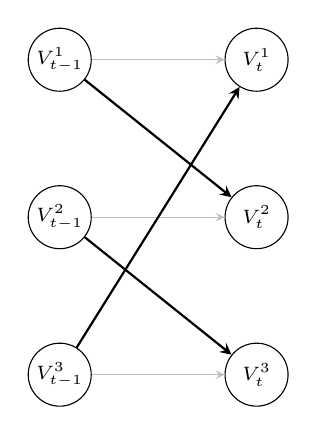
\begin{tikzpicture}[
    every node/.style={draw, circle, minimum size=0.8cm, font=\scriptsize, inner sep=0pt},
    >=stealth,
    ->,
    solidedge/.style={->, thick},
    temporal/.style={->, gray!50},
]

% t-1
\node (V1t1) at (0,4) {$V^1_{t-1}$};
\node (V2t1) at (0,2) {$V^2_{t-1}$};
\node (V3t1) at (0,0) {$V^3_{t-1}$};

% t
\node (V1t) at (2.5,4) {$V^1_t$};
\node (V2t) at (2.5,2) {$V^2_t$};
\node (V3t) at (2.5,0) {$V^3_t$};

% Temporal arrows (gray)
\foreach \i in {1,2,3} {
  \draw[temporal] (V\i t1) -- (V\i t);
}

% Causal edges (example)
\draw[solidedge] (V1t1) -- (V2t);
\draw[solidedge] (V2t1) -- (V3t);
\draw[solidedge] (V3t1) -- (V1t);

\end{tikzpicture}

\vspace{0.3em}
\textbf{(a) Lagged causal graph ($\ell_{\max}=1$)}
\end{minipage}%
\hfill
\begin{minipage}[t]{0.48\textwidth}
\centering
\vspace{0pt}
\renewcommand{\arraystretch}{1.2}
\setlength{\tabcolsep}{6pt}

\textbf{(b) Lagged adjacency tensor slice at lag \(1\)} \\[0.3em]
\(\mathbb{A}^{(0)}\)
\vspace{1.5em}

\begin{tabular}{c|ccc}
 & $V^1_{t-1}$ & $V^2_{t-1}$ & $V^3_{t-1}$ \\
\hline
$V^1_t$ & 0 & 0 & \textbf{1} \\
$V^2_t$ & \textbf{1} & 0 & 0 \\
$V^3_t$ & 0 & \textbf{1} & 0 \\
\end{tabular}

\vspace{1.5em}
%\scriptsize
\textbf{Interpretation:} $\mathbb{A}^{(0)}_{ji}=1$ indicates a directed edge $V^i_{t-1} \!\rightarrow\! V^j_t$.  For $\ell_{\max}=1$, the lag index is $\ell=0$.
\end{minipage}
\vspace{0.5em}
\caption{Illustrative example of a lagged causal graph with \(\ell_{\max}=1\) (left) and its corresponding lagged adjacency tensor (right), for a three-variable case and \(\ell_{\max}=1\). The tensor entry \(\mathbb{A}_{ji\ell_{\max}-\ell}\) indicates whether a directed causal edge from \(V^i_{t-\ell}\) to \(V^j_t\) exists. The LCM performs causal discovery by inferring \(\hat{\mathbb{A}}\), aiming to recover the true adjacency tensor \(\mathbb{A}\).}
\label{fig:lagged-tensor-example}
\end{figure}


\section{Problem Formulation} \label{sec:problem-formulation}

Formally, we seek to construct a \textit{pre-trained neural architecture capable of learning causal graphs from time-series data}. Recall from Section \ref{sec:setting} that the objective of causal discovery is to infer the underlying causal graph \( \mathcal{G} \sim \mathcal{D} \) of a dataset \( \mathcal{D} \sim \mathcal{P}_{\mathcal{D}} \). Our task is to build a \textit{large causal model} (LCM), a foundation model capable of performing causal discovery directly from time-series data, outputting a temporal causal DAG from varying input lengths, domains, and underlying causal mechanisms. Let \(\mathbf{X} = \{ \mathbf{X}_t \}_{t=1}^{n} \in \mathbb{R}^{n \times k}, \quad \mathbf{X}_t = (X_t^1, \ldots, X_t^k) \in \mathbb{R}^k\) denote a multivariate time series with \(n\) timesteps and \(k\) variables. The goal of an LCM is to infer a time-lagged causal graph that captures the directed temporal dependencies among the variables. Specifically:

%\begin{definition}[Large Causal Model]
A \textit{large causal model (LCM)} is a parametric function \(f_\theta\) mapping a multivariate time series \(\mathbf{X}\) to a \textit{lagged causal adjacency tensor}

\begin{equation}
\mathbf{X} \xrightarrow{f_\theta} \hat{\mathbb{A}},
\end{equation}

where \(\hat{\mathbb{A}} \in [0,1]^{k \times k \times \ell_{\max}}\). Each entry \(\hat{\mathbb{A}}_{j,i,\ell_{\max}-\ell}\) represents the model's confidence in the directed causal relationship \(X^i_{t-\ell} \to X^j_t\). The maximum lag \(\ell_{\max}\) is a fixed hyperparameter bounding temporal dependencies, analogous to assumptions in classical methods such as PCMCI \citep{runge2018causal}.
%\end{definition}

Unlike large language models or time-series forecasting foundation models that rely on self-supervision, causal discovery \textit{lacks natural self-supervised signals}. The ground-truth causal structure cannot be inferred from data alone, as it is fundamentally unidentifiable without external assumptions or supervision. Therefore, training follows a \textit{supervised learning scheme}, where pairs of ground truth lagged causal graphs and corresponding time-series samples are provided, generated from a known TSCM. This is illustrated in Figure \ref{fig:lagged-tensor-example}. 

As in neural networks (Figure \ref{fig:nn-train-infer}), two distinct phases are involved: (i) \textit{training}, where the model learns to map time-series data to causal graphs by provided with pairs of time-series data and their corresponding causal graphs in order to minimize its loss function; and (ii) \textit{inference (causal discovery)}, where the model (in constant time), once trained, directly outputs the predicted causal graph for unseen time-series data in the form of a lagged adjacency tensor \(\hat{\mathbb{A}}\), that best approximates the ground truth \(\mathbb{A}\). Figure \ref{fig:lcm-train-infer} conceptually illustrates the training and inference phase.

\begin{figure}[t!]
  \centering
   \makebox[\textwidth][c]{%
    \includegraphics[width=1.3\textwidth]{images/causal-foundation-model.pdf}
  }
  \caption{Training step (left) and inference (causal discovery) step (right) of a large causal model \(f_\theta\), represented as a sequence of blocks. During training, the model learns to map input time-series \(\mathbf{X}\) to causal graphs by minimizing a supervised loss between the predicted graph \(\mathcal{G}_{\text{pred}}\) and ground-truth \(\mathcal{G}_{\text{gt}}\). During inference, the pre-trained model directly outputs \(\mathcal{G}_{\text{pred}}\) for unseen inputs.}
  \label{fig:lcm-train-infer}
\end{figure}

To make the problem well-posed under a supervised learning setting, we assume (i) sufficient overlap between training and test distributions \citep{ke2023learning, stein2024embracing, wu2024sample}, (ii) causal assumptions (described in Table \ref{tab:causal-assumptions}), and (iii) bounded temporal dependencies via fixed \(\ell_{\max}\). This formulation highlights the need for large and diverse training collections of temporal data and their corresponding causal graphs. In practice, \(\hat{\mathbb{A}}\) corresponds to a \textit{soft prediction tensor}: it assigns a confidence score to each potential lagged edge rather than a hard decision. To evaluate performance against the ground truth, these scores are binarized via a thresholding operator \(\hat{\mathcal{G}} = 1\{\hat{\mathbb{A}} \geq \tau\}\) (elaborated in Chapter \ref{chap:training}). Different values of \(\tau\) yield different precision-recall trade-offs, summarized using ROC/AUC and related metrics in Chapter \ref{chap:results}. Additionally, in order to handle samples and TSCMs of varying number of samples, variables and lags, a padding mechanism must be implemented as in conventional foundation models. A thorough discussion of the above is provided in Chapter \ref{chap:architecture}.